\documentclass[10pt,a4paper]{article}

%double si on veut une version prof et une version élève. simple si on veut une seule version.
\newcommand{\buildmode}{double}

\InputIfFileExists{version.tex}{}{}
% Version (définie par le script)
\providecommand{\version}{eleve}

\usepackage{feuilleexo}
\usepackage{schemaevolution}

%%%à modifier à chaque fois

\renewcommand{\niveau}{1M}
\renewcommand{\chapitre}{Fonctions affines}
\renewcommand{\numchap}{0.4} 
\renewcommand{\theme}{Fonctions}

\begin{document}


%\legendeicones

\vspace{-0.3cm}

\begin{prerequis}
\begin{itemize}
    \item Savoir calculer l'image d'une fonction avec la formule.
    \item Savoir à l'aide d'un graphique, retrouver l'image d'un nombre
    \item Savoir retrouver graphiquement les éventuels antécédents d'un nombre par une fonction
    \item Savoir résoudre une équation
    \item Savoir développer une expression
\end{itemize}

\end{prerequis}

\prof{
    Motivation : La première semaine, les élèves ont été réintroduits à la notion de fonction (représentation graphique, tableau de valeur). Les objectifs sont \begin{itemize}
        \item Leur faire comprendre que l'objectif des fonctions n'est pas seulement de décrire, mais aussi de faire des prédictions. Pour cela, ,on commence avec les fonctions affines car ce sont les plus simples.
        \item Introduire des fontions plus complexes (fonctions polynomiales du second degré).
    \end{itemize}
    Début de cours : récupération fonctions affines + rappels de cours : formule algébrique + représentation graphique. Exercices 1 et 2 en application avant d'entamer le cours.
}

\begin{multicols}{2}

\begin{exo}[][]
Pour chacunes des fonctions suivantes, dire celles qui sont affines. Pour celles qui le sont, déterminer leur coefficient directeur et leur ordonnée à l'origine.
\begin{tasks}(2)
\task \(f(x) = \dfrac{1}{x}\)
\task \(g(x) = 5x-4\)
\task \(h(x) = 5x\)
\task \(i(x) = -x+10\)
\task \(j(x) = -10\)
\task \(k(x) = x+\dfrac{7}{3}\)
\task \(l(x) = 2x^2+4\)
\task \(m(x) = \dfrac{x}{2}+ 3\)
\end{tasks}
\end{exo}

\prof{
    Dans un exercice ultérieur, même consigne avec des formules plus difficiles : \(\dfrac{x+3}{2}\), \(2^2x+4\), \(x^2+2x-x^2+5-7\),
}

\begin{exo}
On considère la fonction affine \(k\) définie par \(k(x) = -2x + 1\) où \(x\) est un nombre.
\begin{enumerate}
    \item Compléter le tableau de valeurs de la fonction :
    \begin{center}
        \renewcommand{\arraystretch}{1.5}
        \setlength{\tabcolsep}{1em}
        \begin{tabular}{l|c|c|c|c|c|c}
           \(x\)    & -1 & -0,5 & 0 & 0,5 & 1 & 2 \\ \hline
           \(k(x)\) & & & & & & \\
        \end{tabular}
    \end{center}

    \item Représenter la  fonction dans le repère ci-dessous :
    
    \begin{tikzpicture}
        \begin{axis}[
            axis lines = middle,
            xmajorgrids=true,
            ymajorgrids=true,
            %xlabel = \(x\),
            %ylabel = {\(k(x)\)},
            xmin = -1.7,
            xmax = 2.7,
            ymin = -3.5,
            ymax = 3.5
        ]
        \end{axis}
    \end{tikzpicture}
\end{enumerate}
\end{exo}

\prof{
    S'appliquer sur la correction. Faire comprendre qu'il faut en fait que deux points pour tracer une droite. Faire apparaître le coefficient directeur et l'ordonnée à l'origine.
}

\begin{exo}[][]
    Parmi les quatre droite représentées ci-dessous, une seule peut être la représentation graphique de \(g(x) = 2x-3\). Dire laquelle en justifiant. \begin{multicols}{4}
        \hspace{0.5cm} \(d_1\)\\
        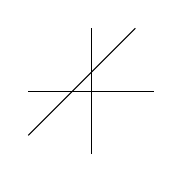
\begin{tikzpicture}[scale=0.8]
            \draw(-1,0)--(1,0);
            \draw(0,-1)--(0,1);
            \draw (-1,-0.7)--(0.7,1);
        \end{tikzpicture}

        \hspace{0.5cm} \(d_2\)\\
        \begin{tikzpicture}[scale=0.8]
            \draw(-1,0)--(1,0);
            \draw(0,-1)--(0,1);
            \draw (-1,0.7)--(0.7,-1);
        \end{tikzpicture}

        \hspace{0.5cm} \(d_3\)\\
        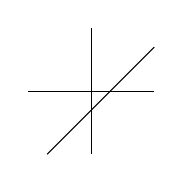
\begin{tikzpicture}[scale=0.8]
            \draw(-1,0)--(1,0);
            \draw(0,-1)--(0,1);
            \draw (-0.7,-1)--(1,0.7);
        \end{tikzpicture}

        \hspace{0.5cm} \(d_4\)\\
        \begin{tikzpicture}[scale=0.8]
            \draw(-1,0)--(1,0);
            \draw(0,-1)--(0,1);
            \draw (-0.7,1)--(1,-0.7);
        \end{tikzpicture}
    \end{multicols}
\end{exo}

\begin{exo}[][]
    Tracer dans le repère ci-dessous les fonctions affines suivantes :\begin{tasks}(2)
        \task \(f(x) = 2x-1\)
        \task \(g(x) = -x+3\)
        \task \(h(x) = -\dfrac{1}{2}x\)
    \end{tasks}
    \begin{tikzpicture}
        \begin{axis}[
            axis lines = middle,
            xmajorgrids=true,
            ymajorgrids=true,
            %xlabel = \(x\),
            %ylabel = {\(k(x)\)},
            xmin = -5.1,
            xmax = 5.1,
            ymin = -5.1,
            ymax = 5.1
        ]
        \end{axis}
    \end{tikzpicture}
\end{exo}

\prof{
    Pour que les élèves comprennent bien la notation de l'exercice qui suit, on peut appeler les droites qu'on a tracé \(\mathcal{D}_{nom de la fonction}\)
}

\begin{exo}
     : 
Retrouver les formules pour chacunes des droites suivantes

    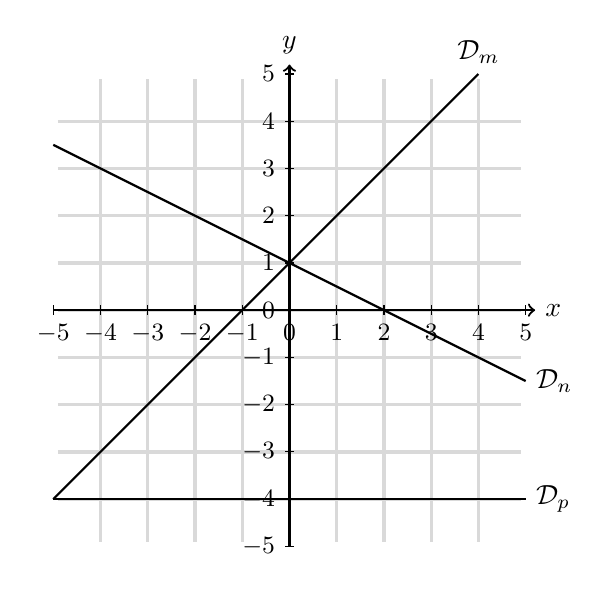
\begin{tikzpicture}[scale=0.6]

  % Grands quadrillages
  \draw[step=1cm, gray!30, very thick] (-4.9,-4.9) grid (4.9,4.9);

  % Axes
  \draw[->, thick] (-5,0) -- (5.2,0) node[right] {$x$};
  \draw[->, thick] (0,-5) -- (0,5.2) node[above] {$y$};

  % Graduations
  \foreach \x in {-5,...,5}
    \draw (\x,0.1) -- (\x,-0.1) node[below] {\small $\x$};

  \foreach \y in {-5,...,5}
    \draw (0.1,\y) -- (-0.1,\y) node[left] {\small $\y$};

  % Droites
  \draw[thick] (-5,-4) -- (4,5) node[above] {$\mathcal{D}_m$};
  \draw[thick] (-5,3.5) -- (5,-1.5) node[right] {$\mathcal{D}_n$};
  \draw[thick] (-5,-4) -- (5,-4) node[right] {$\mathcal{D}_p$};

\end{tikzpicture}
\end{exo}

\begin{exo}[][appro]
    Un plombier facture ses interventions comme indiqué sur le graphique ci-dessous.
    
        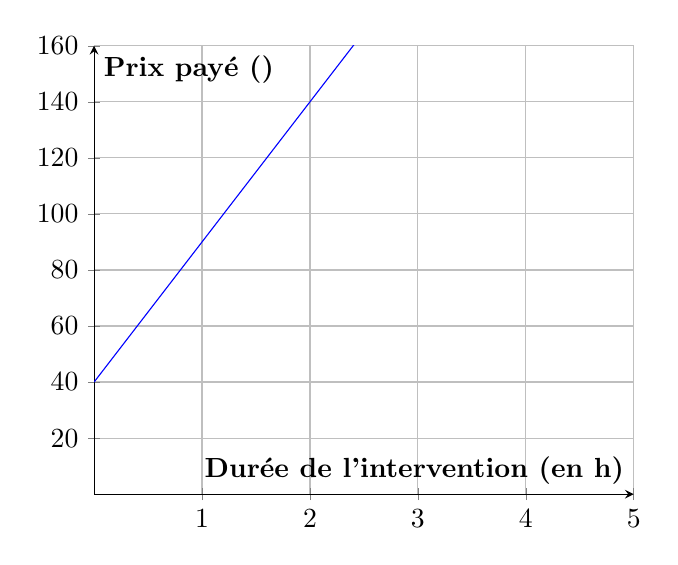
\begin{tikzpicture}
        \begin{axis}[
            axis lines = middle,
            xmajorgrids=true,
            ytick distance = 20,
            ymajorgrids=true,
            xlabel = \textbf{Durée de l'intervention (en h)},
            ylabel = \textbf{Prix payé (\euro)},
            xmin = 0,
            xmax = 5,
            ymin = 0,
            ymax = 160
        ]
        \addplot [
            domain= 0:3, 
            samples=100, 
            color=blue,
            ]
            {50*x+40};
        \end{axis}
    \end{tikzpicture}
    \begin{enumerate}
        \item Combien le plombier facturera-t-il pour 5h de travail ?
        \item Combien le plombier facture-t-il à l'heure ?
        \item Quel est le prix de son déplacement ?
    \end{enumerate}
\end{exo}

\section{Tableaux de signes}

\begin{exo}[][]
    Dresser les tableaux de signe des fonctions affines suivantes :
    \begin{tasks}(2)
        \task \(f(t) = 7t+14\)
        \task \(g(x) = -2x+5\)
        \task \(h(x) = x-4\)
        \task \(i(x) = -x-\dfrac{2}{3}\)
    \end{tasks}
\end{exo}

\prof{
    Obligation de justifier le tableau de signe par  un schéma. Ce sera le cas pour l'interro
}

\begin{exo}[][bac]
    On considère les fonction affines \(f\) et \(g\) définies par \(f(x) = x-4\) et \(g(x) = x+1\).\\
    On considère également la fonction \(m\) définie par \(m(x)=2x^2-6x-8\)
    \begin{enumerate}
        \item Démontrer l'égalité suivante : \(-2(x-4)(x+1) = 2x^2-6x-8\).
        \item En déduire le tableau de signe de la fonction \(m\). Vous pourrez vous aider des tableaux de signe de \(f\) et \(g\).
        \item Tracer la fonction \(m\) entre -2 et 5. Les résultats sont-ils cohérents ?
    \end{enumerate}
\end{exo}

\prof{
    \begin{itemize}
        \item Est-ce que c'est nécessaire de faire tracer la courbe ? Ça prend du temps.
        \item On n'a pas revu comment tracer un tableau de signe à l'aide d'une représentation graphique, est-ce que ça pose problème ?? (C'est pour ça que j'ai rajouté la question 3).
    \end{itemize}
}

\begin{exo}[][bac]
    On considère la fonction \(g\) définie par \(g(x) = 3x^-9x+6\)
    \begin{enumerate}
        \item Développer l'expression \(3(x-2)(x-1)\)
        \item En déduire le tableau de signe de \(g\)
    \end{enumerate}
\end{exo}

\begin{exo}[][bac]
    On considère la fonction \(h\) définie par \(h(t) = t^2+2t+1\)
    \begin{enumerate}
        \item Développer l'expression \((t+1)^2\)
        \item En déduire le tableau de signe de \(h\)
    \end{enumerate}
\end{exo}

\end{multicols}
\end{document}
